%%%%%%%%%%%%%%%%%%%%%%%%%%%%%%%%%%%%%%%%%%%%%%%%%%%%%%%%%%%%
%%% LIVECOMS ARTICLE TEMPLATE FOR BEST PRACTICES GUIDE
%%% ADAPTED FROM ELIFE ARTICLE TEMPLATE (8/10/2017)
%%%%%%%%%%%%%%%%%%%%%%%%%%%%%%%%%%%%%%%%%%%%%%%%%%%%%%%%%%%%
%%% PREAMBLE
\documentclass[9pt,tutorial]{livecoms}
% Use the 'onehalfspacing' option for 1.5 line spacing
% Use the 'doublespacing' option for 2.0 line spacing
% Use the 'lineno' option for adding line numbers.
% Use the "ASAPversion' option following article acceptance to add the DOI and relevant dates to the document footer.
% Use the 'pubversion' option for adding the citation and publication information to the document footer, when the LiveCoMS issue is finalized.
% The 'bestpractices' option for indicates that this is a best practices guide.
% Omit the bestpractices option to remove the marking as a LiveCoMS paper.
% Please note that these options may affect formatting.

\usepackage{lipsum} % Required to insert dummy text
\usepackage[version=4]{mhchem}
\usepackage{siunitx}
\DeclareSIUnit\Molar{M}
\usepackage[italic]{mathastext}
\graphicspath{{figures/}}

%%%%%%%%%% USER INPUT PACKAGES & FUNCTIONS
\usepackage{listings}
\lstset{
	basicstyle=\ttfamily,
	commentstyle={},
	breakatwhitespace=true,
	breaklines=true,
	language=bash
}
\usepackage{pythonhighlight}

%%%%%%%%%%%%%%%%%%%%%%%%%%%%%%%%%%%%%%%%%%%%%%%%%%%%%%%%%%%%
%%% IMPORTANT USER CONFIGURATION
%%%%%%%%%%%%%%%%%%%%%%%%%%%%%%%%%%%%%%%%%%%%%%%%%%%%%%%%%%%%

\newcommand{\versionnumber}{1.0}  % you should update the minor version number in preprints and major version number of submissions.
\newcommand{\githubrepository}{\url{https://github.com/michellab/BioSimSpaceTutorials}}  %this should be the main github repository for this article

%%%%%%%%%%%%%%%%%%%%%%%%%%%%%%%%%%%%%%%%%%%%%%%%%%%%%%%%%%%%
%%% ARTICLE SETUP
%%%%%%%%%%%%%%%%%%%%%%%%%%%%%%%%%%%%%%%%%%%%%%%%%%%%%%%%%%%%
\title{A Suite of Tutorials for the BioSimSpace framework for interoperable biomolecular simulation [Article v\versionnumber]}
% Everyone in alphabetical order other than Lester

\author[1*]{Lester O. Hedges}
\author[]{Sofia Bariami}
\author[2]{Adele Hardie}
\author[3]{Dominykas Lukauskis}
\author[2]{Antonia S.J.S. Mey}
\author[2*]{Julien Michel}
\author[2\authfn{1}]{Jenke Scheen}

%\author[1,2\authfn{1}\authfn{3}]{Firstname Middlename Familyname}
%\author[2\authfn{1}\authfn{4}]{Firstname Initials Surname}
%\author[2*]{Firstname Surname}
\affil[1]{Advanced Computing Research Centre, University of Bristol, UK}
\affil[2]{EaStCHEM School of
Chemistry, University of Edinburgh, UK}
\affil[3]{Department of Chemistry and Institute of Structural and Molecular Biology, University College
London, UK}


\corr{julien.michel@ed.ac.uk}{JM}  % Correspondence emails.  FMS and FS are the appropriate authors initials.
\corr{lester.hedges@bristol.ac.uk }{LH}

\orcid{Lester Hedges}{EEEE-FFFF-GGGG-HHHH}
\orcid{Adele Hardie}{EEEE-FFFF-GGGG-HHHH}
\orcid{Dominykas Lukauskis}{EEEE-FFFF-GGGG-HHHH}
\orcid{Antonia Mey}{0000-0001-7512-5252}
\orcid{Julien Michel}{0000-0003-0360-1760}
\orcid{Jenke Scheen}{EEEE-FFFF-GGGG-HHHH}

%\contrib[\authfn{1}]{These authors contributed equally to this work}
%\contrib[\authfn{2}]{These authors also contributed equally to this work}

\presentadd[\authfn{1}]{Computational and Systems Biology Program, Sloan Kettering Institute, Memorial Sloan Kettering Cancer Center, New York NY, USA}
%\presentadd[\authfn{4}]{Department, Institute, Country}

\blurb{This LiveCoMS document is maintained online on GitHub at \githubrepository; to provide feedback, suggestions, or help improve it, please visit the GitHub repository and participate via the issue tracker.}

%%%%%%%%%%%%%%%%%%%%%%%%%%%%%%%%%%%%%%%%%%%%%%%%%%%%%%%%%%%%
%%% PUBLICATION INFORMATION
%%% Fill out these parameters when available
%%% These are used when the "pubversion" option is invoked
%%%%%%%%%%%%%%%%%%%%%%%%%%%%%%%%%%%%%%%%%%%%%%%%%%%%%%%%%%%%
\pubDOI{10.XXXX/YYYYYYY}
\pubvolume{<volume>}
\pubissue{<issue>}
\pubyear{<year>}
\articlenum{<number>}
\datereceived{Day Month Year}
\dateaccepted{Day Month Year}

%%%%%%%%%%%%%%%%%%%%%%%%%%%%%%%%%%%%%%%%%%%%%%%%%%%%%%%%%%%%
%%% ARTICLE START
%%%%%%%%%%%%%%%%%%%%%%%%%%%%%%%%%%%%%%%%%%%%%%%%%%%%%%%%%%%%

\begin{document}

\begin{frontmatter}
\maketitle

\begin{abstract}
This particular document provides a skeleton illustrating key sections for a Tutorial document.
Please see the sample \texttt{sample-document.tex} in \url{github.com/livecomsjournal/article_templates/templates} for additional information on and examples of using the LiveCoMS LaTeX class.
Here we also assume familiarity with LaTeX and knowledge of how to include figures, tables, etc.; if you want examples, see the sample just referenced.

In your work, in this particular slot, please provide an abstract of no more than 250 words.
Your abstract should explain the main contributions of your article, and should not contain any material that is not included in the main text.
Please note that your abstract, plus the authorship material following it, must not extend beyond the title page or modifications to the LaTeX class will likely be needed.
\end{abstract}

\end{frontmatter}




\section{Introduction}

Here you would explain what problem you are tackling and briefly motivate your work.

In this particular template, we have removed most of the usage examples which occur in \texttt{sample-document.tex} to provide a minimal template you can modify; however, we retain a couple of examples illustrating more unusual features of our templates/article class, such as the checklists, and information on algorithms and pseudocode.

Keep in mind, as you prepare your manuscript, that you should plan for a representative image  which will be used to highlight your article on the journal website and publications. Usually, this would be one of your figures, but it must also be uploaded separately upon article submission. We give specific guidelines for this image on the journal website in the section on article submission (see \url{https://livecomsjournal.github.io/authors/policies/index.html#article-submission}).

Additionally, for well-formatted manuscripts, we recommend that you let LaTeX handle figure/table placement for you as much as possible, so please avoid specifying strenuous float instructions like `[h!]` and `[H]` as much as possible.

\subsection{Scope}

Tutorials should endeavor to cover the specific task at hand, and also highlight how the steps might need to be modified (or additional care might need to be taken at particular points) to handle more general cases.

The scope of the tutorial, as well as the expected proficiencies / outcomes for researchers who complete the tutorial, should be clearly defined.
This will often happen in a specific section or subsection in the article itself.

\section{Prerequisites}

Here you would identify prerequisites/background knowledge that are assumed by your work, as well as any software/license requirements.

\subsection{Background knowledge}
Tutorials should clearly define what concepts or abilities researchers will need to complete the tutorial (e.g., some proficiency in Python; experience with Jupyter notebooks; knowledge of classical MD; etc).

\subsection{Software/system requirements}
Tutorials should clearly define what system and/or software requirements the researcher will need to complete the tutorial (e.g., VMD version 1.9 or newer, AMBER, etc.). Tutorials requiring specific software packages must provide instructions and files for the referenced version of the software.

\section{Content and links}

A tutorial will normally draw on additional files and materials; clearly indicate where and how these are available, with links, and how they are being archived for the long-term and maintained so they stay current.
You will likely want to reference your GitHub repository as a central point to access all of this information, and then the GitHub repository may link out to other content as needed.

%TODO Fix layout issues 
\subsection{Tutorial 1: Introduction}
%Author: Lester Hedges Email:~~ lester.hedges@bristol.ac.uk

\hypertarget{biosimspace}{%
\section{BioSimSpace}\label{biosimspace}}

The companion notebook for this section can be found
\href{https://github.com/michellab/BioSimSpaceTutorials/blob/4844562e7d2cd0b269cead56562ec16a3dfaef7c/01_introduction/01_introduction.ipynb}{here}.

\hypertarget{introduction}{%
\subsection{Introduction}\label{introduction}}

Welcome to this workshop on \href{https://biosimspace.org}{BioSimSpace},
an \emph{interoperable} Python framework for biomolecular simulation. In
this introductory session you will learn:

\begin{itemize}
\tightlist
\item
  What are the key concepts behind BioSimSpace.
\item
  How to set up molecular systems ready for simulation.
\item
  How to configure and run a range of molecular dynamics protocols using
  different simulation engines.
\item
  How to write interoperable workflow components and run them in a
  variety of ways.
\end{itemize}

\hypertarget{what-is-biosimspace}{%
\subsection{What is BioSimSpace?}\label{what-is-biosimspace}}

As a computational chemist, you are likely overwhelmed by the amount of
different software packages that are available to you. Having choice is
a good thing, but too much can become a burden. I'm sure you have all
come across at least one of the following:

\begin{itemize}
\tightlist
\item
  I know how to solve the problem with package X but I want to use
  package Y.
\item
  How can I share my script with a collaborator who doesn't use the same
  software stack?
\item
  How can I take advantage of the best tool for the job for different
  parts of my workflow?
\item
  How can I compare methodology / results between simulation engines?
\end{itemize}

Solving these problems is the core goal of BioSimSpace. The wealth of
fantastic software in our community is a real asset but
\emph{interoperability} is currently a problem. Since there is no point
reinventing the wheel, BioSimSpace is not an attempt to produce yet
another molecular simulation package that reproduces all of the
functionality from existing programs. This would result in just another
tool for you to learn, along with yet another set of standards and
formats. Instead, BioSimSpace is essentially just a set of \emph{shims},
or bits of \emph{glue}, that connect together existing software
packages, allowing you to interact with them using a consistent Python
interface.

\hypertarget{why-biosimspace}{%
\subsection{Why BioSimSpace?}\label{why-biosimspace}}

By using BioSimSpace you will be less reliant on the use of brittle
scripts to connect different software packages together. BioSimSpace
builds on top of existing and open Python tools within the biomolecular
community, e.g. \href{https://www.rdkit.org/}{RDKit},
\href{http://openmm.org/}{OpenMM},
\href{https://github.com/openforcefield/openff-toolkit}{Open Force
Field}. As such, you are able to leverage the power of other packages,
with which you may already be familiar, and to mix-and-match
functionality where required.

With BioSimSpace you will be able to:

\begin{itemize}
\tightlist
\item
  Write generic workflow components \emph{once} in a package-agnostic
  language.
\item
  Run the same script from the command-line, Jupyter, or within a
  workflow engine.
\item
  Use the most suitable package that is availabe on your computer.
\item
  Continue using your favourite package X but be able to share scripts
  with your collaborator who prefers package Y.
\item
  Be able to take advantage of new software packages and hardware
  resources as and when they become available.
\end{itemize}

\hypertarget{what-can-biosimspace-do}{%
\subsection{What can BioSimSpace do?}\label{what-can-biosimspace-do}}

BioSimSpace provides a suite of packages with a range of different
functionality.

At present:

\begin{itemize}
\tightlist
\item
  File conversion:
  \href{https://biosimspace.org/api/index_IO.html}{BioSimSpace.IO}
\item
  Parameterisation:
  \href{https://biosimspace.org/api/index_Parameters.html}{BioSimSpace.Parameters}
\item
  Solvation:
  \href{https://biosimspace.org/api/index_Solvent.html}{BioSimSpace.Solvent}
\item
  Molecular dynamics:
  \href{https://biosimspace.org/api/index_Protocol.html}{BioSimSpace.Protocol},
  \href{https://biosimspace.org/api/index_Process.html}{BioSimSpace.Process},
  \href{https://biosimspace.org/api/index_MD.html}{BioSimSpace.MD}
\item
  Free-energy perturbation:
  \href{https://biosimspace.org/api/index_Align.html}{BioSimSpace.Align},
  \href{https://biosimspace.org/api/index_FreeEnergy.html}{BioSimSpace.FreeEnergy}
\item
  Metadynamics:
  \href{https://biosimspace.org/api/index_Metadynamics.html}{BioSimSpace.Metadynamics}
\item
  Trajectory handling:
  \href{https://biosimspace.org/api/index_Trajectory.html}{BioSimSpace.Trajectory}
\item
  Interactive visualisation:
  \href{https://biosimspace.org/api/index_Notebook.html}{BioSimSpace.Notebook}
\item
  Workflow components:
  \href{https://biosimspace.org/api/index_Gateway.html}{BioSimSpace.Gateway}
\end{itemize}

\hypertarget{key-concepts}{%
\subsection{Key concepts}\label{key-concepts}}

Before getting started it's worth spending a little time covering a few
of the key concepts of BioSimSpace.

\hypertarget{file-conversion}{%
\subsubsection{File conversion}\label{file-conversion}}

While, broadly speaking, the different molecular dynamics engines offer
a similar range of features, their interfaces are quite different. This
makes it hard to take expertise in one package and immediately apply it
to another. At the heart of this problem is the incompatibility between
the molecular file formats used by the different packages. While they
all contain the same information, i.e.~how atoms are laid out in space
and how they interact with each other, the structure of the files is
very different. In order to provide interoperability betwen packages we
will need to be able to read and write many different file formats, and
be able to interconvert between them too.

Let's import the BioSimSpace Python package and see what we can do. For
convenience, we'll rename the package to BSS to save us typing:

\begin{Shaded}
\begin{Highlighting}[]
\ImportTok{import}\NormalTok{ BioSimSpace }\ImportTok{as}\NormalTok{ BSS}
\end{Highlighting}
\end{Shaded}

To see what file formats are supported by BioSimSpace, execute the cell
below.

\begin{Shaded}
\begin{Highlighting}[]
\NormalTok{BSS.IO.fileFormats()}
\end{Highlighting}
\end{Shaded}

\begin{verbatim}
['Gro87', 'GroTop', 'MOL2', 'PDB', 'PRM7', 'PSF', 'RST', 'RST7']
\end{verbatim}

Note that these refer to specific file \emph{formats}, rather than file
\emph{extensions}. BioSimSpace doesn't care about file extensions, it's
the \emph{contents} of the file that's important.

If you aren't familiar with a particular format, you can get more
information as follows, e.g.:

\begin{Shaded}
\begin{Highlighting}[]
\NormalTok{BSS.IO.formatInfo(}\StringTok{"GroTop"}\NormalTok{)}
\end{Highlighting}
\end{Shaded}

\begin{verbatim}
'Gromacs Topology format files.'
\end{verbatim}

The \texttt{BSS.IO.readMolecules} function is used to read molecular
information from file. We've provided some example input files for you
in the \texttt{inputs} directory. Let's take a look at some of these.

\begin{Shaded}
\begin{Highlighting}[]
\OperatorTok{!}\NormalTok{ls inputs}
\end{Highlighting}
\end{Shaded}

\begin{verbatim}
1jr5.crd  1jr5.top  ala.crd  kigaki.gro  methanol.pdb
1jr5.pdb  2JJC.pdb  ala.top  kigaki.top
\end{verbatim}

The \texttt{ala.crd} and \texttt{ala.top} files define a solvated
alanine dipeptide system in AMBER format. Execute the cell below to see
part of the topology file:

\begin{Shaded}
\begin{Highlighting}[]
\OperatorTok{!}\NormalTok{head }\OperatorTok{-}\NormalTok{n }\DecValTok{20}\NormalTok{ inputs}\OperatorTok{/}\NormalTok{ala.top}
\end{Highlighting}
\end{Shaded}

\begin{verbatim}
%VERSION  VERSION_STAMP = V0001.000  DATE = 06/30/15  11:44:23                  
%FLAG TITLE                                                                     
%FORMAT(20a4)                                                                   
ACE                                                                             
%FLAG POINTERS                                                                  
%FORMAT(10I8)                                                                   
    1912       9    1902       9      25      11      43      24       0       0
    2619     633       9      11      24      13      21      20      10       1
       0       0       0       0       0       0       0       1      10       0
       0
%FLAG ATOM_NAME                                                                 
%FORMAT(20a4)                                                                   
HH31CH3 HH32HH33C   O   N   H   CA  HA  CB  HB1 HB2 HB3 C   O   N   H   CH3 HH31
HH32HH33O   H1  H2  O   H1  H2  O   H1  H2  O   H1  H2  O   H1  H2  O   H1  H2  
O   H1  H2  O   H1  H2  O   H1  H2  O   H1  H2  O   H1  H2  O   H1  H2  O   H1  
H2  O   H1  H2  O   H1  H2  O   H1  H2  O   H1  H2  O   H1  H2  O   H1  H2  O   
H1  H2  O   H1  H2  O   H1  H2  O   H1  H2  O   H1  H2  O   H1  H2  O   H1  H2  
O   H1  H2  O   H1  H2  O   H1  H2  O   H1  H2  O   H1  H2  O   H1  H2  O   H1  
H2  O   H1  H2  O   H1  H2  O   H1  H2  O   H1  H2  O   H1  H2  O   H1  H2  O   
H1  H2  O   H1  H2  O   H1  H2  O   H1  H2  O   H1  H2  O   H1  H2  O   H1  H2  
\end{verbatim}

Let's now read the molecules from file. The
\texttt{BSS.IO.readMolecules} function automatically
\href{https://en.wikipedia.org/wiki/Glob_(programming)}{globs} the
passed string, so wildcard matching can be used to determine the files.
(Here the asterisk matches any characters, i.e.~we are reading
\emph{all} files in the \texttt{inputs} directory with \texttt{ala} as
the file prefix.)

\begin{Shaded}
\begin{Highlighting}[]
\NormalTok{system }\OperatorTok{=}\NormalTok{ BSS.IO.readMolecules(}\StringTok{"inputs/ala.*"}\NormalTok{)}
\end{Highlighting}
\end{Shaded}

N.B. We could have explictly specified each file using a list of
strings.

Note that we don't have to specify anything about the file format.
BioSimSpace actually reads the files with \emph{all} of its inbuilt
parsers in parallel. If a parser fails to read the file then it is
immediately rejected and we move on to the next. As long as all of the
files that are read contain a consistent topology, then BioSimSpace will
be able to read them.

To see what file formats are associated with the system, run:

\begin{Shaded}
\begin{Highlighting}[]
\NormalTok{system.fileFormat()}
\end{Highlighting}
\end{Shaded}

\begin{verbatim}
'PRM7,RST7'
\end{verbatim}

As expected, BioSimpace has detected that these were AMBER format
topology and coordinate files.

The molecules are now loaded into a \texttt{System} object. BioSimSpace
objects are thin wrappers around the equivalent objects from
\href{https://github.com/michellab/Sire}{Sire}. For those that are
familiar with Sire, you can get always access the underlying object
directly using \texttt{system.\_sire\_object}. This \emph{private}
member is hidden from the user. Sire provides an extremely powerful and
flexible set of tools for molecular manipulation and editing. While
BioSimSpace directly exposes only a small subset of this functionality
to the user, the full power of Sire is always easily available when
needed.

We can query how many molecules there are as follows:

\begin{Shaded}
\begin{Highlighting}[]
\NormalTok{system.nMolecules()}
\end{Highlighting}
\end{Shaded}

\begin{verbatim}
631
\end{verbatim}

To see how many water molecules there are:

\begin{Shaded}
\begin{Highlighting}[]
\NormalTok{system.nWaterMolecules()}
\end{Highlighting}
\end{Shaded}

\begin{verbatim}
630
\end{verbatim}

To search for all nitrogen atoms in residues named \texttt{ALA}:

\begin{Shaded}
\begin{Highlighting}[]
\NormalTok{system.search(}\StringTok{"element N and resname ALA"}\NormalTok{)}
\end{Highlighting}
\end{Shaded}

\begin{verbatim}
<BioSimSpace.SearchResult: nResults=1>
\end{verbatim}

Create a new system using from the first 10 and last molecule in the
system:

\begin{Shaded}
\begin{Highlighting}[]
\NormalTok{new_system }\OperatorTok{=}\NormalTok{ (system[:}\DecValTok{10}\NormalTok{] }\OperatorTok{+}\NormalTok{ system[}\OperatorTok{-}\DecValTok{1}\NormalTok{]).toSystem()}
\end{Highlighting}
\end{Shaded}

N.B. Information from the topology file pertaining to the molecular
force field are stored internally as computer algebra expressions,
allowing us to mathematically interconvert between different
representations of the terms when writing to a different format. If
desired, you could even edit the system to create your own unique force
field parameters, although this beyond the scope of this tutorial.

Now that we have a molecular system, let's write it back to disk in a
different format. Unsurprisingly, this is done using the
\texttt{BSS.IO.saveMolecules} function. Execute the cell below to write
the system to GROMACS format coordinate and topology files.

\begin{Shaded}
\begin{Highlighting}[]
\NormalTok{BSS.IO.saveMolecules(}\StringTok{"ala"}\NormalTok{, system, [}\StringTok{"Gro87"}\NormalTok{, }\StringTok{"GroTop"}\NormalTok{])}
\end{Highlighting}
\end{Shaded}

\begin{verbatim}
['/home/lester/Code/BioSimSpaceTutorials/01_introduction/ala.gro',
 '/home/lester/Code/BioSimSpaceTutorials/01_introduction/ala.top']
\end{verbatim}

Run the cell below to examine the start of the GROMACS topology file.

\begin{Shaded}
\begin{Highlighting}[]
\OperatorTok{!}\NormalTok{head }\OperatorTok{-}\NormalTok{n }\DecValTok{20}\NormalTok{ ala.top}
\end{Highlighting}
\end{Shaded}

\begin{verbatim}
; Gromacs Topology File written by Sire
; File written 05/06/21  14:17:35
[ defaults ]
; nbfunc      comb-rule       gen-pairs      fudgeLJ     fudgeQQ
  1           2               yes            0.5         0.833333

[ atomtypes ]
; name      at.num        mass      charge   ptype       sigma     epsilon
     C           6   12.010700    0.000000       A    0.339967    0.359824
    CT           6   12.010700    0.000000       A    0.339967    0.457730
    CX           6   12.010700    0.000000       A    0.339967    0.457730
     H           1    1.007940    0.000000       A    0.106908    0.065689
    H1           1    1.007940    0.000000       A    0.247135    0.065689
    HC           1    1.007940    0.000000       A    0.264953    0.065689
    HW           1    1.007940    0.000000       A    0.000000    0.000000
     N           7   14.006700    0.000000       A    0.325000    0.711280
     O           8   15.999400    0.000000       A    0.295992    0.878640
    OW           8   15.999400    0.000000       A    0.315061    0.636386

[ moleculetype ]
\end{verbatim}

\hypertarget{topology-preservation}{%
\subsubsection{Topology preservation}\label{topology-preservation}}

One of the other pitfalls of working with different molecular simulation
engines is that they often have quirks regarding naming conventions and
atom ordering. This means that what you get back from a given program
might not be the same as what you put in, making it tricky to
cross-reference parts of the system that are of specific interest.

N.B. Differerent naming conventions are one of the hardest problems with
interoperability.

BioSimSpace tries to preserve the intial molecular topology during any
interaction with external tools so that it can be used as a consistent
reference. For example, while we might need to rename the water topology
to match the conventions of a particular molecular dynamics engine, we
always copy the updated coordinates from a simulation back into the
original system so that the naming that the user gets back is unchanged.

Another common topology feature that can be lost is chain identifiers.
For example, a \href{https://www.rcsb.org/}{Protein Data Bank} file
might contain labels for chains, but these would be lost during
parameterisation with the
\href{https://ambermd.org/AmberTools.php}{AmberTools} suite since it has
no internal concept of chains.

As an example, consider the following PDB file:

\begin{Shaded}
\begin{Highlighting}[]
\NormalTok{system_pdb }\OperatorTok{=}\NormalTok{ BSS.IO.readMolecules(}\StringTok{"inputs/1jr5.pdb"}\NormalTok{)}
\end{Highlighting}
\end{Shaded}

This is read as a single molecule containing two chains:

\begin{Shaded}
\begin{Highlighting}[]
\BuiltInTok{print}\NormalTok{(}\SpecialStringTok{f"mols = }\SpecialCharTok{\{}\NormalTok{system_pdb}\SpecialCharTok{.}\NormalTok{nMolecules()}\SpecialCharTok{\}}\SpecialStringTok{, chains = }\SpecialCharTok{\{}\NormalTok{system_pdb}\SpecialCharTok{.}\NormalTok{nChains()}\SpecialCharTok{\}}\SpecialStringTok{"}\NormalTok{)}
\end{Highlighting}
\end{Shaded}

\begin{verbatim}
mols = 1, chains = 2
\end{verbatim}

The molecule in the system has a topology but no force field
information, as we can see by querying the \emph{properties} of the
underlying Sire object:

\begin{Shaded}
\begin{Highlighting}[]
\NormalTok{system_pdb[}\DecValTok{0}\NormalTok{]._sire_object.propertyKeys()}
\end{Highlighting}
\end{Shaded}

\begin{verbatim}
['alt_loc',
 'beta_factor',
 'coordinates',
 'element',
 'insert_code',
 'formal_charge',
 'fileformat',
 'occupancy',
 'is_het']
\end{verbatim}

After parameterising the molecule with an AMBER protein force field, we
end up with the following system:

\begin{Shaded}
\begin{Highlighting}[]
\NormalTok{system_amber }\OperatorTok{=}\NormalTok{ BSS.IO.readMolecules([}\StringTok{"inputs/1jr5.crd"}\NormalTok{, }\StringTok{"inputs/1jr5.top"}\NormalTok{])}
\end{Highlighting}
\end{Shaded}

In contrast, this is read as a two molecules with zero chains:

\begin{Shaded}
\begin{Highlighting}[]
\BuiltInTok{print}\NormalTok{(}\SpecialStringTok{f"mols = }\SpecialCharTok{\{}\NormalTok{system_amber}\SpecialCharTok{.}\NormalTok{nMolecules()}\SpecialCharTok{\}}\SpecialStringTok{, chains = }\SpecialCharTok{\{}\NormalTok{system_amber}\SpecialCharTok{.}\NormalTok{nChains()}\SpecialCharTok{\}}\SpecialStringTok{"}\NormalTok{)}
\end{Highlighting}
\end{Shaded}

\begin{verbatim}
mols = 2, chains = 0
\end{verbatim}

Molecules in the parameterised system contain a different set of
properties, including those pertaining to the force field.

\begin{Shaded}
\begin{Highlighting}[]
\NormalTok{system_amber[}\DecValTok{0}\NormalTok{]._sire_object.propertyKeys()}
\end{Highlighting}
\end{Shaded}

\begin{verbatim}
['intrascale',
 'bond',
 'angle',
 'fileformat',
 'atomtype',
 'LJ',
 'charge',
 'connectivity',
 'forcefield',
 'mass',
 'coordinates',
 'treechain',
 'gb_radii',
 'ambertype',
 'improper',
 'element',
 'parameters',
 'gb_screening',
 'gb_radius_set',
 'dihedral']
\end{verbatim}

If we want to preserve the topology of the original molecule, yet add
the updated properties from the molecules in the new system, then we can
make it \emph{compatible}. BioSimSpace provides functionality to do this
for you:

\begin{Shaded}
\begin{Highlighting}[]
\CommentTok{# Extract the original molecule.}
\NormalTok{new_mol }\OperatorTok{=}\NormalTok{ system_pdb[}\DecValTok{0}\NormalTok{]}

\CommentTok{# Make it compatible with the new system, i.e. add new properties while}
\CommentTok{# preserving the topology.}
\NormalTok{new_mol.makeCompatibleWith(system_amber)}
\end{Highlighting}
\end{Shaded}

N.B. This is done implicitly whenever calling any BioSimSpace
parameterisation function.

Let's now check the number of chains in the new molecule, as well as the
properties that are associated with it.

\begin{Shaded}
\begin{Highlighting}[]
\BuiltInTok{print}\NormalTok{(}\SpecialStringTok{f"chains = }\SpecialCharTok{\{}\NormalTok{new_mol}\SpecialCharTok{.}\NormalTok{nChains()}\SpecialCharTok{\}}\SpecialStringTok{"}\NormalTok{)}
\NormalTok{new_mol._sire_object.propertyKeys()}
\end{Highlighting}
\end{Shaded}

\begin{verbatim}
chains = 2





['formal_charge',
 'is_het',
 'intrascale',
 'bond',
 'angle',
 'fileformat',
 'atomtype',
 'LJ',
 'charge',
 'connectivity',
 'forcefield',
 'alt_loc',
 'mass',
 'beta_factor',
 'coordinates',
 'occupancy',
 'treechain',
 'gb_radii',
 'ambertype',
 'improper',
 'element',
 'insert_code',
 'gb_screening',
 'gb_radius_set',
 'dihedral']
\end{verbatim}

\input{LIVECOMS/01_introduction/02_molecular_setup}
\input{LIVECOMS/01_introduction/03_molecular_dynamics}
\input{LIVECOMS/01_introduction/04_writing_nodes}
\input{LIVECOMS/01_introduction/05_running_nodes}

\subsection{Tutorial 2: Funnel Meta-Dynamics}
\hypertarget{funnel-metadynamics-tutorial}{%
\label{funnel-metadynamics-tutorial}}
\hypertarget{Introduction}{%
\subsubsection{Introduction}\label{Introduction}}

Funnel metadynamics (fun-metaD) is a molecular dynamics-based method
that calculates the absolute binding free energy (ABFE) between a small
organic ligand and a protein. It uses an enhanced sampling method called
metadynamics, that speeds up the molecular processes of interest by
periodically adding small amounts of bias. To best separate the bound
and unbound phases, as well as increase the rate of convergence, the
exploration of the ligand in 3D space is limited by funnel-shaped
restraints.

This tutorial paper will describe how to setup and analyse fun-metaD
simulations. The main paper that explains what fun-metaD is by
\href{https://www.pnas.org/content/110/16/6358}{Limogelli \emph{et al}
2013} but in this tutorial I will describe the
\href{https://www.ncbi.nlm.nih.gov/pmc/articles/PMC7467642/}{Rhys
\emph{et al} 2020} and
\href{https://pubs.acs.org/doi/10.1021/acs.jcim.6b00772}{Saleh \emph{et
al} 2017} implementation. The main difference between the two
implementations is the functional form of the funnel restraints: the
original fun-metaD relied on a cone and a cylinder joined to make a
funnel using a step function, while the new implementation uses a single
sigmoid function. The Limogelli implementation also requires the protein
to be realigned with a reference structure to keep the funnel strictly
in place over the binding site, which hurts the performance. The
implementation I will describe here allows the funnel to move with the
protein.

Up to now, one of the biggest drawbacks to using fun-metaD for
large-scale absolute binding free energy (ABFE) calculations was the
difficulty in setting up the simulations. It's hard to know where the
funnel should be defined, how big it needs to be, what each of the
sigmoid function parameters should be set to, along with the chore of
writting PLUMED files, where each protein and ligand system will have
slightly different atom IDs.

BioSimSpace has made this easier, automatically defining the funnel
using abstract features of the protein cavity, assigning the relevant
atom IDs, suggesting reasonable default funnel parameters and allowing
the visualisation of the funnel restraints inside a Jupyter Notebook.
All this leads to a quicker setup and much faster automation of large
ABFE screening campaigns.

By the end of this tutorial you should know: 1. The basics of what
fun-metaD does. 2. How to setup fun-metaD simulations and how to
visualise the funnel restraints. 3. How to analyse the results of a
fun-metaD simulation.

\hypertarget{the-theory}{%
\subsubsection{The Theory}\label{the-theory}}

Metadynamics is an enhanced sampling method that biases a simulation
along a chosen set of reaction coordinates, or as MetaD practitioners
call them, collective variables (CVs). This bias is deposited at defined
time intervals and takes the shape of a Gaussian potential.
Investigation of drug binding should involve at least one CV, distance
from the drug molecule to the protein, where the distance between them
can be biased, causing the drug to unbind. However, that single distance
is degenerate, meaning many different configurations of the drug in 3D
space will not be described by that single distance. It also involves
the exploration of a very large volume, hindering convergence.

Fun-metaD gets around both of these problems, restricting the
exploration by using funnel-shaped restraints and reducing degeneracy by
using two CVs - `projection' and `extent'. See Figure \ref{fig:funnel}.

\begin{figure}[htp]
\includegraphics[width=\linewidth]{02_funnel_metad/figures/figure1.jpeg}
\caption{Visualised funnel restraints.}
\label{fig:funnel}
\end{figure}

The restraints that limit the pp.ext CV follow a sigmoid function:

\begin{equation}
S = h\left(\frac{1}{1+b^{b(i-x)}}\right) + f
\end{equation}

where, S is the maximal distance from the axis, at pp.proj = i, h is the
`wall\_width', f is the `wall\_buffer', b is the `beta\_cent' (the
steepness at the inflection point), x is the `s\_cent' (the inflection
point as a value of pp.proj). The exploration along the pp.proj is
limited by the `lower\_wall' and `upper\_wall' parameters. The funnel's
radius at the narrow end is equal to `wall\_buffer'. `P0' and `Px' are
the points that define the funnel's vector. From now on I'll refer to
them as p0 and p1, respectively.

Clearly, there is still some degeneracy in the CVs - the plane
perpendicular to the projection axis is a one dimensional representation of a two dimensional space. However, this is a good compromise between having sufficient accuracy for describing the binding of a
ligand and the tolerable simulation slowdown of using only two CVs.

In ordered to have a good separation between the bound and unbound phases for the ABFE estimations, the funnel needs to point `out', with the narrow end in the solvent,
and away from any protein residues. BSS funnel assignment code does this pretty well. Most of the vectors it picks for defining the p0 and p1 points are good enough for an unobstructed exit path for the ligand. It is still a good idea to check, especially for new protein systems, by
having a look using the funnel visualisation functionality within BSS.

In terms of deciding on how big the radius of funnel should be, it varies on a case-by-case basis.
In general, the funnel will need to be smaller than it seems necessary. The metadynamics code tracks the exploration of the center of mass of the ligand, so the volume that the small molecule will explore is much bigger than it looks intuitively. There is usually only one binding site and the funnel should enclose only it, excluding other protein
features, by setting a small `wall\_width'. This really helps with
convergence by preventing the drug molecule from exploring irrelevant
regions in the free energy surface (FES). Other funnel parameters do not influence matters
that much and the default settings will suffice in most situations.

\hypertarget{visualising-restraints}{%
\subsubsection{Visualising funnel restraints}\label{Visualising the funnel restraints}}

Before we go on to setting up the metadynamics simulation, we can quickly check the funnel restraints using BSS. Load the fully solvated HSP90 protein-ligand system (PDBID:2WI2) and the suggested funnel restraints:

\begin{python}
import BioSimSpace as BSS

# Load the system.
system = BSS.IO.readMolecules(
            ["input_files/solvated.prm7",
             "input_files/solvated.rst7"])

# Create the funnel parameters.
p0, p1 = BSS.Metadynamics.CollectiveVariable.makeFunnel(
            system)

# Define the collective variable.
funnel_cv = BSS.Metadynamics.CollectiveVariable.Funnel(
            p0, p1)

# Create a view.
view = BSS.Metadynamics.CollectiveVariable.viewFunnel(
            system, funnel_cv)

view.system()

\end{python}

Figure \ref{fig:fun-hsp90} below is what you should see in your Jupyter Notebook. 

\begin{figure}[htp]
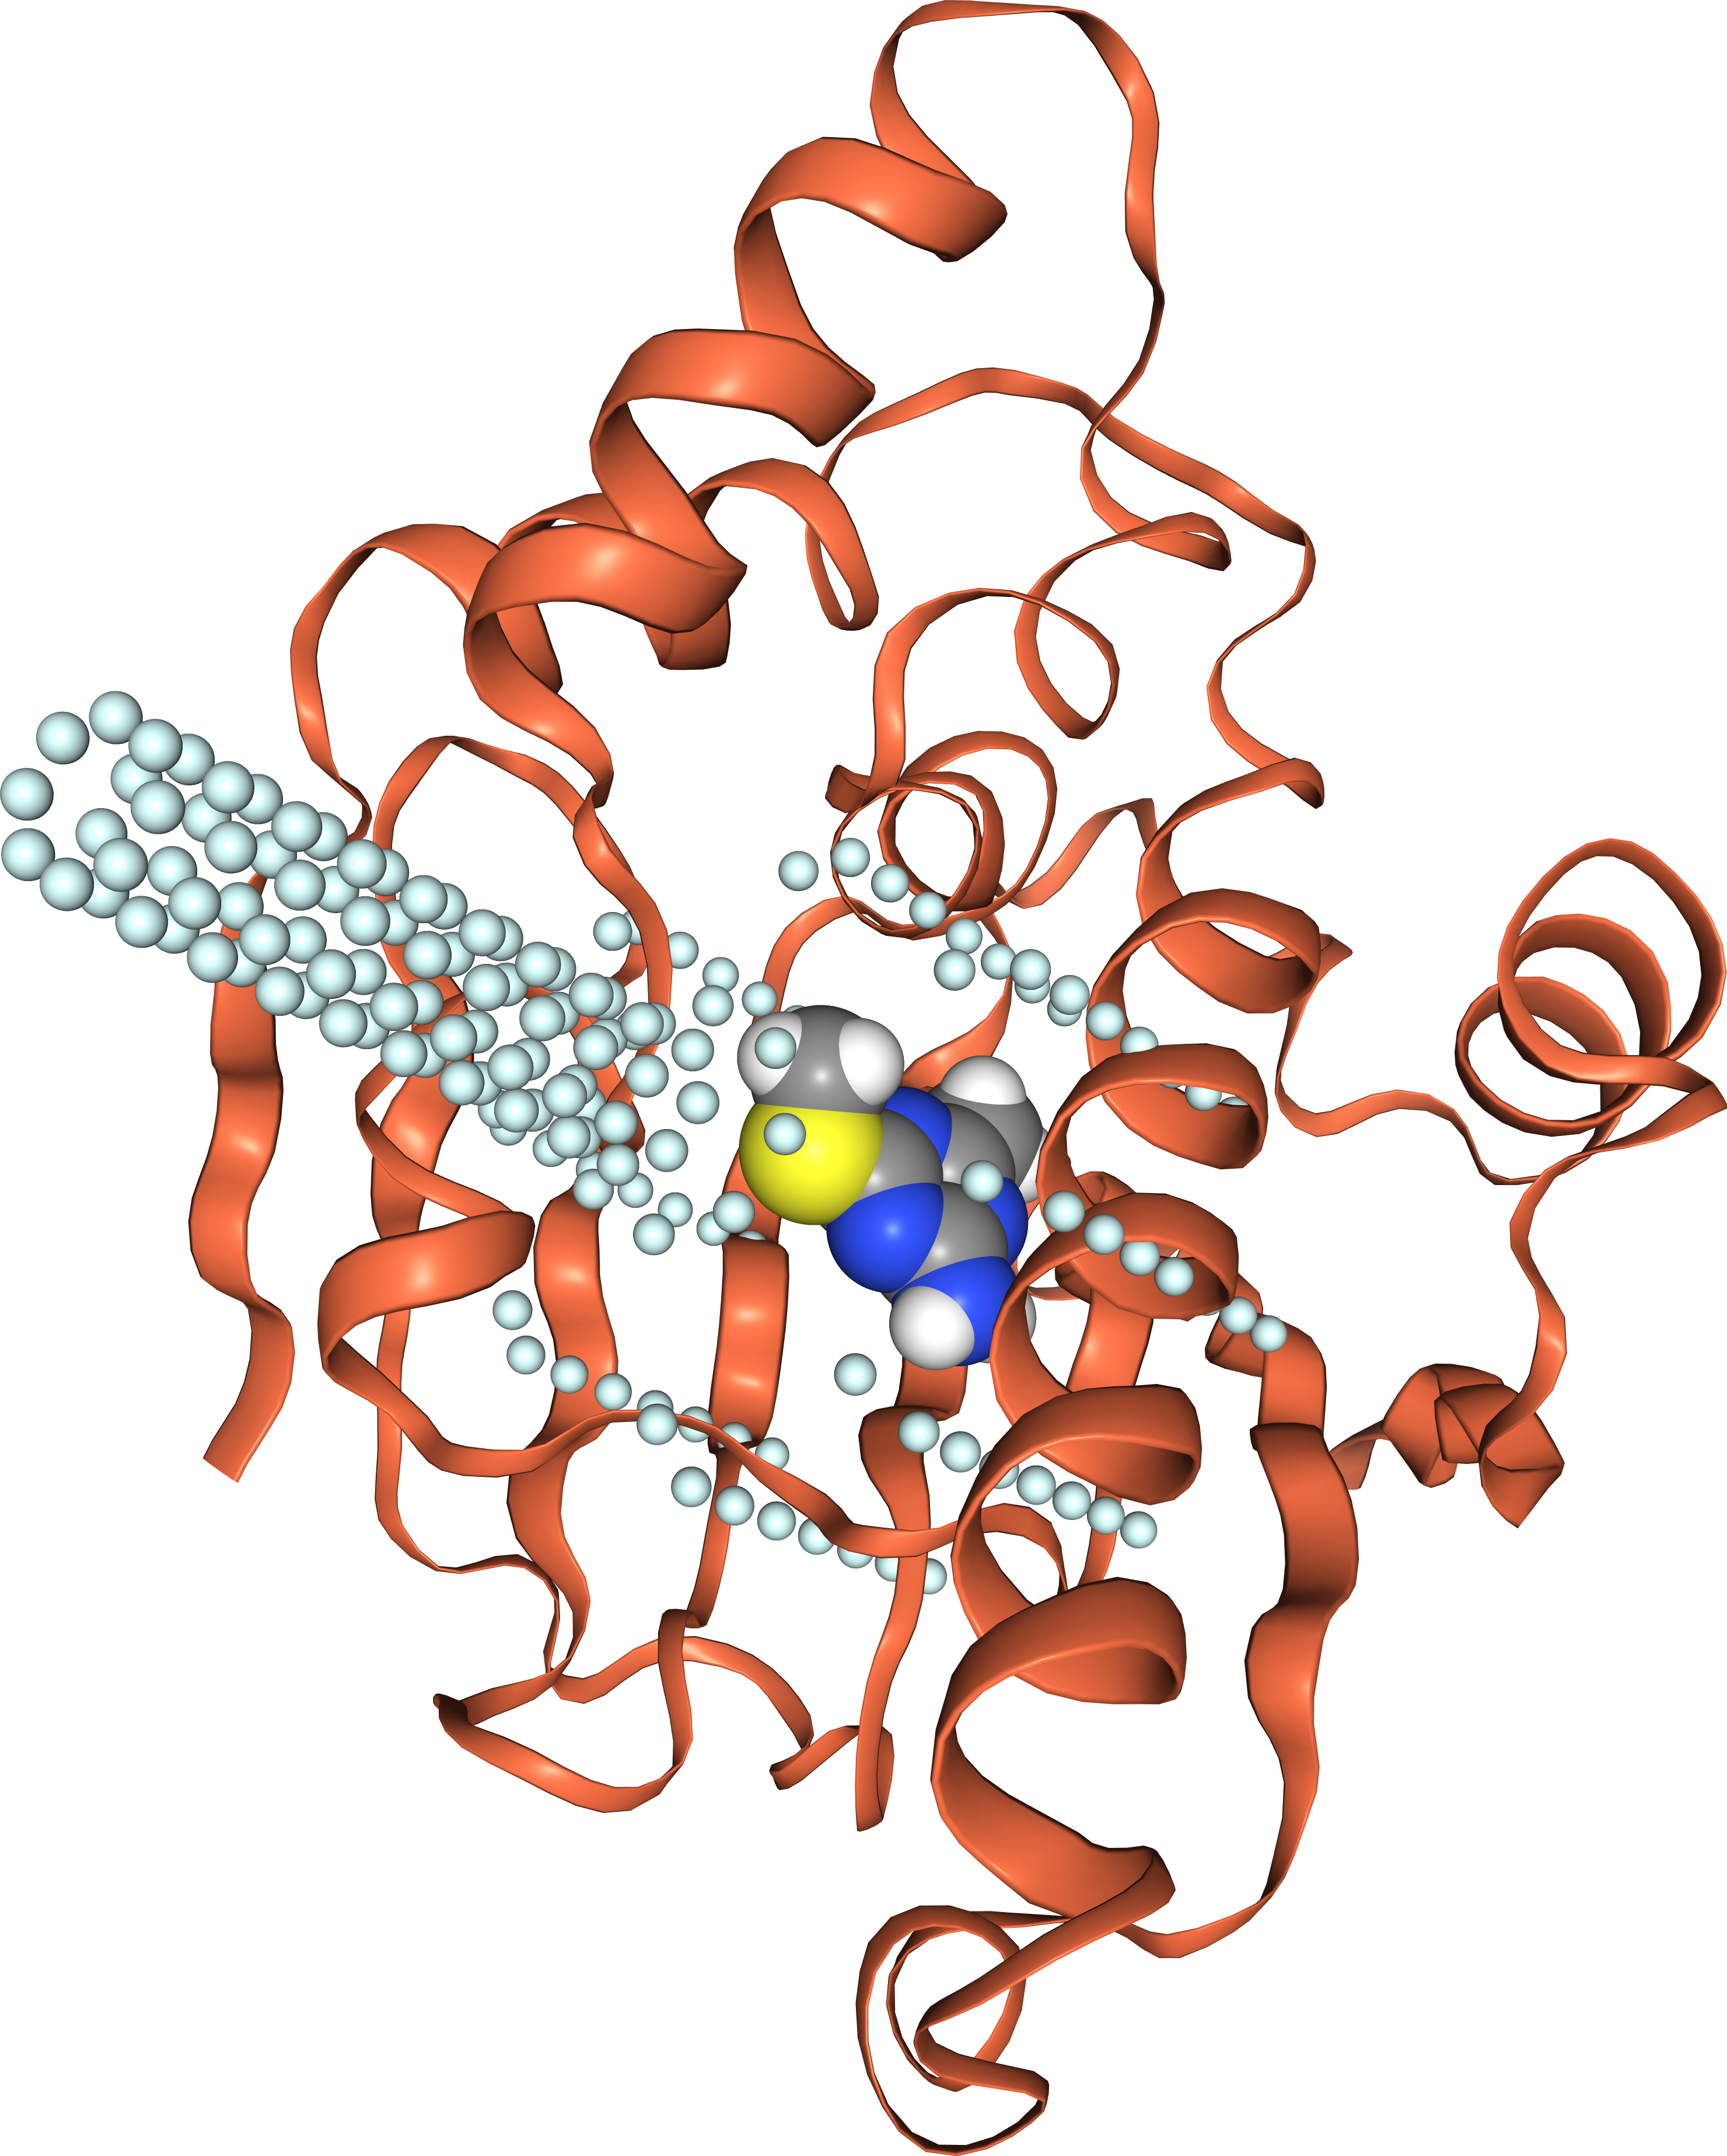
\includegraphics[width=\linewidth]{02_funnel_metad/figures/fun-hsp90.png}
% \caption{Visualised funnel restraints.}
\label{fig:fun-hsp90}
\end{figure}

The funnel vector is clearly pointing out into the solvent, with no protein residues blocking the way. The default radius is sufficient to encompass the binding site, excluding rest of the protein.

\hypertarget{setting-up-the-simulation}{%
\subsubsection{Setting up the simulation}\label{setting-up-the-simulation}}

For this part, open the \texttt{02\_bss-fun-metad-tutorial.ipynb}
notebook.

\hypertarget{analysis}{%
\subsubsection{Analysing fun-metaD simulations}\label{analysis}}

Open the \texttt{03\_bss-fun-metad-analysis.ipynb} notebook.

\subsection{Tutorial 3: Steered Molecular Dynamics \& Markov State Modeling}
\subsubsection{Introduction}
The drug discovery process is mainly concerned with finding small molecules that interact with a target and have a therapeutic effect. However, a large source of failure in these endeavours has been the undruggability of targets.\cite{sMD_druggability} In these cases typical drug-like molecules cannot be used for various reasons, such as due to the shape (or absence) of the target pocket (e.g. in case of protein-protein interactions)\cite{sMD_scott-ppi-2016} or the nature of the active site (e.g. if it is highly charged).\cite{sMD_ptp-rev-druggability} An alternative to directly targeting the active site is allosteric inhibition, which is a way of affecting enzyme function at one site through binding at a different one, through a network of residue interactions \cite{sMD_Motlagh-allostery,sMD_Verkhivker-allostery} This allows the choice of pockets more suitable for small molecule drug design.

An example undruggable target is protein tyrosine phosphatase 1B (PTP1B), which has a charged active site. It is a negative regulator of insulin signalling\cite{sMD_ptp1b-diabetes} and is an attractive target for type II diabetes.\cite{sMD_Wiesman} The function of PTP1B depends on the conformation of its WPD loop, which can be closed (active) or open (inactive) (Figure \ref{fig:ptp1b}). It will be used as an example system for this tutorial.

\begin{figure}[htp]
\includegraphics[width=\linewidth]{03_steered_md/figures/open-close.png}
\caption{The WPD loop of PTP1B, in two conformations: open (yellow, PDB ID: 2HNP) and closed (red, PDB ID: 1SUG).}
\label{fig:ptp1b}
\end{figure}

Since allosteric inhibition is more complex than just physically blocking the active site, knowledge of good binding is not sufficient. An assessment of whether the binder is affecting protein function is required as well. One way of evaluating this is through populations of active and inactive conformations. Here this is achieved through Markov State Models (MSMs). \cite{sMD_Prinz} An MSM is an \textit{n $\times$ n} transition matrix that described the probability of the system transitioning to some state \textit{j} given that it is in state \textit{i}, after a given lag time $\tau$. The system is treated as memoryless, i.e. the transition probabilities do not depend on any previous states, only the current one.\cite{sMD_Husic-msm} This means model building only requires local equilibrium and can make use of multiple shorter trajectories. MSMs can thus model longer timescales without the associated computational cost.\cite{sMD_Prinz}

For the MSMs to more accurately represent statistical ensemble of protein configurations, enhanced sampling methods may be used. Steered molecular dynamics (sMD) is the focus of this tutorial. The WPD loop of PTP1B opens and closes on a $\mu$s timescale,\cite{sMD_Choy-Timescales} and therefore this transition is not observed on conventional computational timescales. sMD introduces a bias potential that is added to the Hamiltonian, thus biasing the simulation towards a specified value of a chosen collective variable (CV). This can be done via PLUMED, which is integrated in BioSimSpace.\cite{sMD_steeredMD,sMD_plumed-2} Once a larger conformational space has been explored via sMD, snapshots of various conformations can be used as starting points for equilibrium MD simulations. The trajectory data from those is then used to build an MSM (Figure \ref{fig:ensemble-protocol}).

\begin{figure}[htp]
\includegraphics[width=\linewidth]{03_steered_md/figures/ensemble-md-protocol.png}
\caption{The steps of using enhanced sampling methods to gather data for statistical analysis of protein conformation ensemble. (1) Run steered MD along some collective variable (CV); (2) Extract snapshots that evenly sample available conformational space; (3) Run equilibrium MD simulations using extracted coordinates as seeds; (4) construct an MSM using trajectory data from step 3.}
\label{fig:ensemble-protocol}
\end{figure}

\subsubsection{Running sMD using BioSimSpace}
sMD using BioSimSpace is very similar to regular production, starting with importing it and reading a parameterised and equilibrated system:
\begin{python}
import BioSimSpace as BSS
system = BSS.IO.readMolecules(["data/system.prm7", 
                                "data/system.rst7"])
\end{python}

The main requirement for sMD is to set up the CV. In this case, RMSD of all heavy atoms for residues of the WPD loop (179-185) will be used. For this, a reference structure is needed, as well as specific atom indices to be used for RMSD calculation:
\begin{python}
reference = BSS.IO.readMolecules("data/reference.pdb")
            .getMolecule(0)
rmsd_indices = []
for residue in reference.getResidues():
    if 178<=residue.index()<=184:
        for atom in residue.getAtoms():
            if atom.element()!="Hydrogen (H, 1)":
                rmsd_indices.append(atom.index())
rmsd_cv = BSS.Metadynamics.CollectiveVariable.RMSD(
                system, reference, 0, rmsd_indices)
\end{python}

One thing to note when dealing with RMSD between two different structures, is that the atoms may not be in the same order. For example, atom 1 in system in this case is a hydrogen, whereas in reference it is an oxygen. BioSimSpace takes care of this by matching up the atoms in the system to the atoms in the reference. The requirements for the reference structure are that all atoms found in reference.pdb must also exist in system. They are matched by residue number and atom name. For example, if the reference structure has an atom named CA in residue 1, there must be an equivalent in the system, and they will be mapped together.

BioSimSpace has a separate protocol for steering. To set one up, steering intervals and restraints need to be specified. Generally sMD consists of four stages (Table \ref{sMD-structure}). The end times of these stages are set:
\begin{python}
start = 0* BSS.Units.Time.nanosecond
apply_force = 4 * BSS.Units.Time.picosecond
steer = 150 * BSS.Units.Time.nanosecond
relax = 152 * BSS.Units.Time.nanosecond
\end{python}

\begin{table}
    \caption{sMD structure. Initially, the force is applied over a few picoseconds, followed by the steering (the bulk of the simulation). The force is removed at the end for system relaxation.}
    \label{sMD-structure}
    \begin{tabular}{|c|c|c|}
    \hline
       Stage  &  CV value  &  Force  \\
       \hline
        1. start  &  initial value  &  none \\
        \hline
        2. apply force  &  initial value  &  specified force  \\
        \hline
        3. steering  &  specified value  &  specified force  \\
        \hline
        4. relaxation  &  specified value  & none  \\
        \hline
    \end{tabular}
\end{table}

The length of the steering step is the most important here and will depend on the system, the steering force constant, and the magnitude of the change sMD is supposed to accomplish. The restraints specify the expected end CV values and the force constant ($\vec{s}_0$(t) and $\kappa$(t)) at each step created above. The protocol can then be created:
\begin{python}
nm = BSS.Units.Length.nanometer
restraint_1 = BSS.Metadynamics.Restraint(
                rmsd_cv.getInitialValue(), 0)
restraint_2 = BSS.Metadynamics.Restraint(
                rmsd_cv.getInitialValue(), 3500)
restraint_3 = BSS.Metadynamics.Restraint(0*nm, 3500)
restraint_4 = BSS.Metadynamics.Restraint(0*nm, 0)
protocol = BSS.Protocol.Steering(rmsd_cv, 
        [start, apply_force, steer, relax], 
        [restraint_1, restraint_2, restraint_3, restraint_4], 
        runtime=152*BSS.Units.Time.nanosecond)
\end{python}

This protocol can be used to create a process. At the moment sMD in BioSimSpace is supported with AMBER and GROMACS, and requires an installation of either of these MD engines patched with PLUMED.
\begin{python}
process = BSS.Process.Amber(system, protocol)
process.getConfig()
\end{python}
\begin{lstlisting}[columns=flexible]
['Production.',
 ' &cntrl',
...
 '  pres0=1.01325,',
 '  plumed=1,',
 '  plumedfile="plumed.dat,',
 ' /']
\end{lstlisting}

The lines plumed=1 and plumedfile="plumed.dat" are what specify that PLUMED will be used. The process can now be started to run steered MD.

\subsubsection{sMD trajectory analysis and seeded MD}
The sMD increases the number of starting conformations available for the MSM data. The next step is to save frames with various WPD loop conformations and use those as starting points for seeded MD simulations. As the sMD simulation is run, the CV values are saved to a \textbf{COLVAR} file. It can be plotted to assess whether the sMD simulation has been successful. An example is shown in Figure \ref{fig:rmsd}.

\begin{figure}[htp]
    \centering
    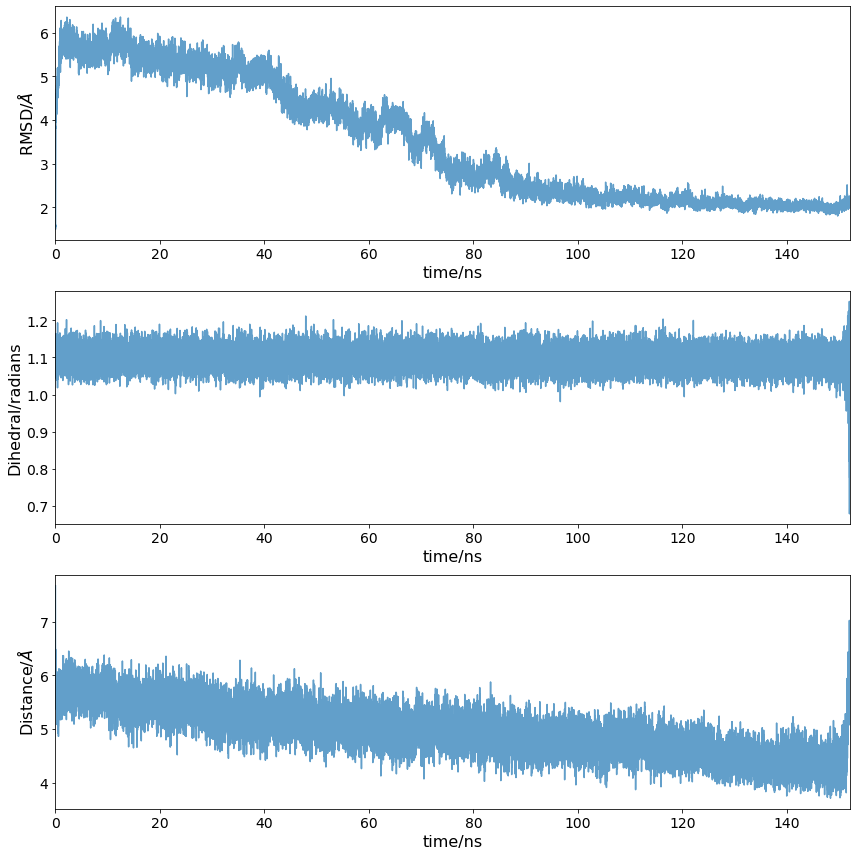
\includegraphics[width=\linewidth]{03_steered_md/figures/COLVAR_all.png}
    \caption{RMSD change throughout an sMD simulation. As the simulation progresses, the WPD loop RMSD gets closer and closer to the closed loop crystal structure (i.e. the loop is being closed).}
    \label{fig:rmsd}
\end{figure}

Once suitable frames have been chosen (here 100 evenly spaces snapshots are used as they sample the entire RMSD range), they can be saved as PDBs with BioSimSpace:
\begin{python}
for i, index in enumerate(frames):
    frame = BSS.Trajectory.getFrame(
    trajectory='/home/user/Documents/PTP1B/steering.nc', 
    topology = '/home/user/Documents/PTP1B/system.prm7', 
    index=int(index))
    BSS.IO.saveMolecules('data/snapshot_{i+1}',
                        frame, 'pdb')
\end{python}

These PDBs are then used as starting points for an array of 100 ns equilibrium MD simulations. As this requires a lot of computational resources, it is recommended to run this on an HPC cluster.

\subsubsection{Markov State Models}
There is a lot to consider when building MSMs, and the method is not covered in this tutorial. Here the python library \href{http://emma-project.org/latest/}{PyEMMA} was used, which has extensive examples and documentation. The exact method of building the following MSM is also provided in the jupyter notebook \textbf{03\_msm\_full.ipynb}.

The results of the data obtained from the results described above is shown in Figure \ref{fig:msm}. sMD was used to steer the WPD loop of PTP1B from open to closed and from closed to open, and 100 snapshots were extracted from each trajectory (200 in total). These were then used as starting points for 100 ns equilibrium MD simulations. The model indicates that this particular way of modelling PTP1B with peptide substrate results in catalytically active conformations 2\% of the time. Returning to the idea of allosteric inhibition, if a second model, built for a system including an allosteric binder of interest, showed a decrease in active conformation probability, it would suggest that this binder has inhibition potential. 

\begin{figure}[htp]
    \centering
    \includegraphics[width=\linewidth]{03_steered_md/figures/msm_final.png}
    \caption{The population of three metastables states as predicted by the MSM.}
    \label{fig:msm}
\end{figure}
\subsection{Tutorial 4: Free Energy Perturbation}
%TODO MERGE IN TUTORIALS AT https://github.com/michellab/bssccpbiosim2022
% [From antonia Mey, Anna Herz, Finlay Clark)]
%%%%%%%%%%%%%%%%%%%%%%%%%%%%%%%%%%%%%%%%%%%%%%%%%%%%%%%%%%%%%%%%%%%%%%%%%%%%%%%%%%%%%%%%%%%
%%%%%%%%%%%%%%%%%%%%%%%%%%%%%%%%%%%%%%%%%%%%%%%%%%%%%%%%%%%%%%%%%%%%%%%%%%%%%%%%%%%%%%%%%%%
%%%%%%%%%%%%%%%%%%%%%%%%%%%%%%%%%%%%%%%%%%%%%%%%%%%%%%%%%%%%%%%%%%%%%%%%%%%%%%%%%%%%%%%%%%%
%%%%%%%%%%%%%%%%%%%%%%%%%%%%%%%%%%%%%%%%%%%%%%%%%%%%%%%%%%%%%%%%%%%%%%%%%%%%%%%%%%%%%%%%%%%
%%%%%%%%%%%%%%%%%%%%%%%%%%%%%%%%%%%%%%%%%%%%%%%%%%%%%%%%%%%%%%%%%%%%%%%%%%%%%%%%%%%%%%%%%%%
%%%%%%%%%%%%%%%%%%%%%%%%%%.  WRITE YOUR CHAPTER CONTENTS BELOW.  %%%%%%%%%%%%%%%%%%%%%%%%%%
%%%%%%%%%%%%%%%%%%%%%%%%%%%%%%%%%%%%%%%%%%%%%%%%%%%%%%%%%%%%%%%%%%%%%%%%%%%%%%%%%%%%%%%%%%%
%%%%%%%%%%%%%%%%%%%%%%%%%%%%%%%%%%%%%%%%%%%%%%%%%%%%%%%%%%%%%%%%%%%%%%%%%%%%%%%%%%%%%%%%%%%
%%%%%%%%%%%%%%%%%%%%%%%%%%%%%%%%%%%%%%%%%%%%%%%%%%%%%%%%%%%%%%%%%%%%%%%%%%%%%%%%%%%%%%%%%%%

\subsubsection{Introduction}


Computational chemists can support structure-activity relationship
studies in medicinal chemistry by making computer models that can
predict binding affinity of ligands to proteins. One of the most popular
techniques for this is Free Energy Perturbation (FEP), which relies on
simulation alchemical transformations of ligands in a congeneric series,
simulating them both in a protein target and in just a waterbox.
Relative free energies of binding ($\Delta\Delta$G in kcal/mol) can then be computed
by simply subtracting the $\Delta$G (in protein) and the $\Delta$G (in water). Some
introductory reading is recommended. \cite{mey2020best, cournia_allen_sherman_2017, kuhn_firth-clark_tosco_mey_mackey_michel_2020}

This tutorial will outline the steps needed to:

\begin{itemize}
\item
  Select a series of transformations to simulate using LOMAP
\item
  Use BioSimSpace to set up files needed for a standard FEP run in both
  SOMD and GROMACS
\item
  Run FEP using BioSimSpace on a computing cluster
\item
  Process FEP simulation results
\item
  Compile all FEP results locally and perform data analyses
\end{itemize}

For this tutorial we will be using TYK2, a common benchmarking set in
the FEP field, first used by Schrödinger in their
\href{https://pubs.acs.org/doi/abs/10.1021/ja512751q}{2015 FEP+ paper}.

\begin{figure}[htp]
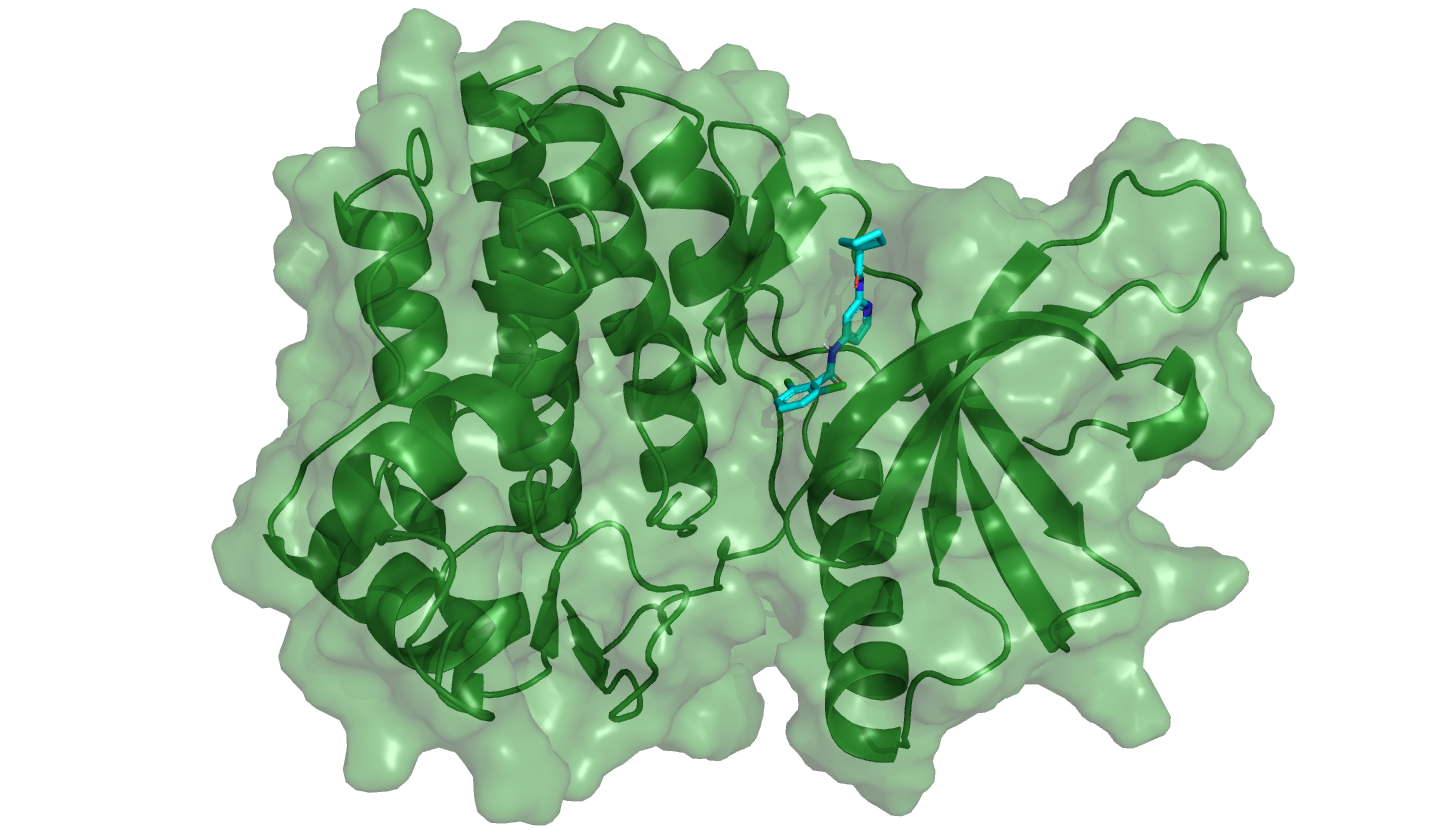
\includegraphics[width=\linewidth]{04_fep/inputs/tut_imgs/tyk2_protlig.png}
\caption{Tyrosine kinase 2 (TYK2) structure with bound ligand
(ejm\_48).}
\label{tyk2_bound_fig}
\end{figure}


Typically in FEP the goal is to predict free energies of binding for a
collection of ligands (normally 10-20). Although methods exist (such as
absolute FEP) that can predict these energies directly (i.e. $\Delta$Gbind),
these are often complicated and computationally expensive. (relative)
FEP uses a basic rule in thermodynamics that dictates that, given a
thermodynamic cycle, the net energy must always be 0. FEP allows users
to compute the $\Delta\Delta$G of binding between two ligands through this mechanism
(see figure \ref{thermodynamic_cycle_fig}).

\begin{figure}[htp]
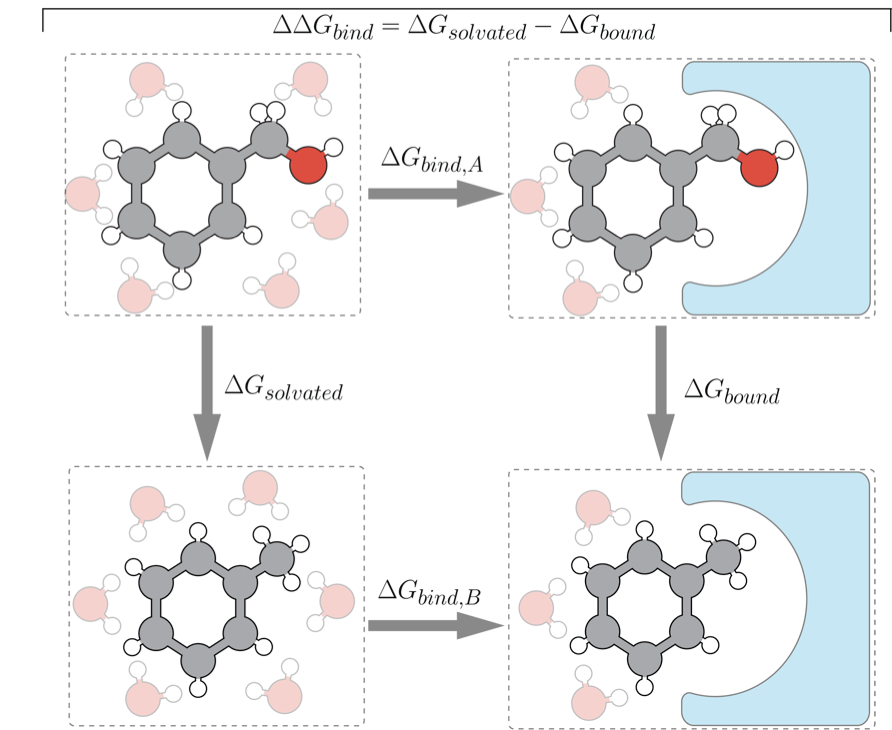
\includegraphics[width=\linewidth]{04_fep/inputs/tut_imgs/therm_cycle.png}
\caption{Thermodynamic cycle that allows FEP practicioners to
compute relative energies of binding. Because the difference between the
vertical legs equals the difference between the horizontal legs, we can
circumvent predicting $\Delta$G$_{bind}$ directly, but instead compute $\Delta\Delta$G$_{bind}$ by
transforming between two ligands in both the solvated and bound phase.}
\label{thermodynamic_cycle_fig}
\end{figure}

Because \emph{relative} energies are calculated, pairs of ligands have to be transformed into one another in both the fee and bound phase (hence the name free energy \emph{perturbation}. Typically, smaller (i.e. fewer heavy atoms) transformations are more reliable which means
that for a ligand series it is recommended to selectively make combinations of
ligands to cover the whole series. In FEP, this is done this using
\emph{perturbation networks}, typically generated by FEP softwares.
Although generating these networks can be done by hand, it is typically
better to do it programmatically to save time and create more optimal networks
(transformation reliability does not depend just on transformation size,
but also on a series of other unfavourable moiety transformations).

\subsubsection{Setting up a FEP calculation using BioSimSpace}

BioSimSpace allows users to set up and run a FEP calculation with just a
few lines of code (and input files). First, BioSimSpace is imported and
and input structures are read:

\begin{python}
import BioSimSpace as BSS
ligand_1 = BSS.IO.readMolecules("ligand_1.mol2")[0]
ligand_2 = BSS.IO.readMolecules("ligand_2.mol2")[0]
protein = BSS.IO.readMolecules("protein.pdb")[0]
\end{python}

\noindent Input molecules are parameterised using Amber-style force fields:

\begin{python}
ligand_1 = BSS.Parameters.gaff2(ligand_1).getMolecule()
ligand_2 = BSS.Parameters.gaff2(ligand_2).getMolecule()
protein = BSS.Parameters.ff14sb(protein).getMolecule()
\end{python}

\noindent We support a variety of other force fields as well. Because one ligand is transforming to the other, they need to be
well aligned. This can be done by:

\begin{python}
atom_mapping = BSS.Align.matchAtoms(ligand_1, ligand_2)
ligand_1 = BSS.Align.rmsdAlign(ligand_1, ligand_2, 
                                     atom_mapping)
\end{python}

\noindent Now a `merged' molecule (i.e. a molecule that we can
manipulate in a way such that the endpoints are either input ligands) has to be made. Adding this merged structure into the protein structure can be done simply by addition; the complete system can then be solvated.

\begin{python}
merged = BSS.Align.merge(ligand_1, ligand_2)
system = merged + protein
system_solvated = BSS.Solvent.tip3p(molecule=system, 
                box=3*[10*BSS.Units.Length.nanometer])
\end{python}

\noindent At which point all structures necessary for a FEP run are created. A FEP protocol can be set by:

\begin{python}
protocol = BSS.Protocol.FreeEnergy()
\end{python}

\noindent Note that calling no arguments sets the default FEP protocol. BioSimSpace can set up all necessary files by:

\begin{python}
freenrg_free = BSS.FreeEnergy.Relative(solvated, 
                        protocol, work_dir="output")
freenrg_bound = BSS.FreeEnergy.Relative(system_solvated, 
                        protocol, work_dir="output")
\end{python}

\noindent Running the free and bound FEP calculations is done by:

\begin{python}
freenrg_free.run() 
freenrg_bound.run() 
\end{python}
\noindent After simulations have finished we can retrieve the free energies and subtract them to get the relative binding free energy:
\begin{python}
pmf_bound, overlap_bound = freenrg_bound.analyse()
pmf_free,  overlap_free  = freenrg_free.analyse()

free_nrg_binding = \
BSS.FreeEnergy.Relative.difference(pmf_bound, pmf_free)
\end{python}

\noindent Note that this only makes sense on a workstation with GPUs or GPU cloud resources or a GPU cluster. If the code is run as above, each $\lambda$ window simulation is run sequentially which is not very efficient.

\subsubsection{Workflow of a BioSimSpace FEP pipeline}

Because a single FEP simulation typically takes hours to run on a
single GPU (depending on settings and hardware), FEP is usually run on a
computing cluster (or HPC/ cloud service). This allows practitioners to
run many simulations at the same time, turning an FEP pipeline into a
process that takes just several days (or even fewer) instead of weeks (or
even more).

Given a protein input file and a series of ligand input files, we will
be using a Jupyter Notebook that uses LOMAP to generate a perturbation
network for us. This notebook will also write all files necessary to
further prepare our FEP simulations. Because preparing ligands and
proteins for FEP can already require some heavy computation, this will
be the first process that will run on a cluster. Then, after running and
processing the FEP outputs, we can download the results back to our
local workstation. There, the analysis notebook uses FreeEnergyAnalysis
to process FEP predictions and generate plots.

\begin{figure}[htp]
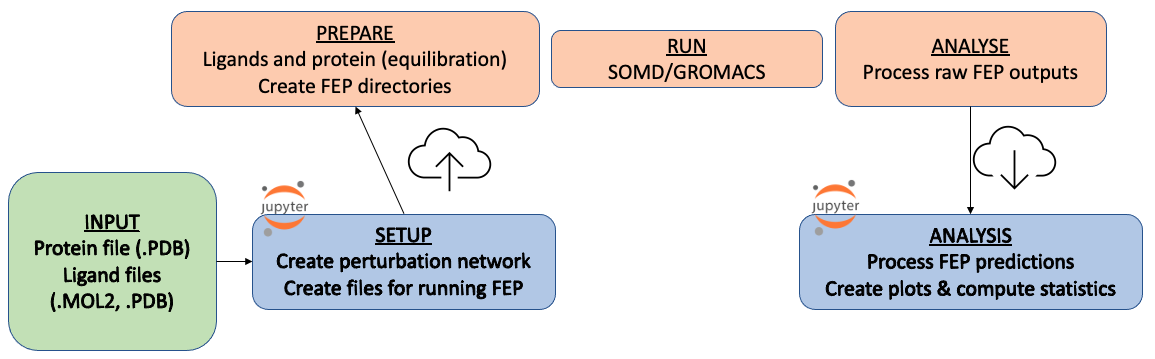
\includegraphics[width=\linewidth]{04_fep/inputs/tut_imgs/fep_pipeline.png}
\caption{Schematic of the FEP pipeline in this tutorial. Whereas blue boxes
represent notebooks run on a local machine, orange boxes represent
python scripts run sequentially on a computing cluster.}
\label{fep_pipeline_fig}
\end{figure}


\subsubsection{Generating a perturbation network to run FEP on a congeneric series of ligands}

For this step, open the jupyter notebook \textbf{setup\_fep.ipynb}. If
you would like to use your own ligands and protein, you can put these in
\texttt{inputs/ligands/} and \texttt{inputs/protein/}, respectively.

After running all the cells in this notebook, the folder
\texttt{./execution\_model/} will contain everything needed to run FEP
in parallel on your cluster. To move this folder to your cluster, you
can use for instance SCP:

\begin{lstlisting}
$ scp -r execution_model uname@cluster.address:/path/to/folder
\end{lstlisting}

\noindent \emph{Note: if a computing cluster shares its file system with the local workstation the above step is not needed.}


\subsubsection{Running FEP on a computing cluster using
BioSimSpace}

The folder \texttt{./execution\_model/} contains several scripts and
folders, of which the most important are:

\begin{itemize}
\item
  \texttt{processFEP-slurm.sh} and \texttt{processFEP-lsf.sh}: running
  either of these scripts will submit all simulation jobs (depending on the
  cluster setup). Note that there are several parameters at the top of
  these scripts that have to be set (by e.g. a system administrator)
  that will inform BioSimSpace of all relevant paths to software
  dependencies and other important matters.
\item
  \texttt{./scripts/} contains all necessary scripts to run FEP with
  BioSimSpace. Advanced users can tweak more settings in these.
\end{itemize}

If everything has been set up correctly, running:

\begin{lstlisting}
$ bash processFEP-slurm.sh
\end{lstlisting}

will start the whole FEP job submission (for SLURM clusters). First, all systems will be
prepared, then run and then analysed (see figure \ref{fep_pipeline_fig}). When jobs finish, FEP predictions will be written to \texttt{./outputs/SOMD/summary.csv} (in case of SOMD
engine). Logfiles for seeing process outputs can be found in
\texttt{./logs/}. Additionally, perturbations that were simulated
successfully will have an \emph{overlap matrix} figure saved to
\texttt{./logs/} (in case of SOMD); these can be checked to check if perturbations were likely to be reliable per simulation leg. \cite{mey2020best}

For the final analysis, only \texttt{./outputs/SOMD/summary.csv} is required. Thus, this file has to be downloaded back to the local workstation; using SCP again (from the workstation, i.e. not logged into the cluster):

\begin{lstlisting}
$ scp uname@cluster.address:/path/to/folder\ /outputs/SOMD/summary.csv .
\end{lstlisting}


\subsubsection{Analysing FEP results}

For this step, open the jupyter notebook \textbf{analyse\_fep.ipynb}.
Running cells in this notebook will generate typical FEP figures
(barplots and scatterplots); if you have missing or failed
perturbations, the script should be able to work out an optimal
prediction (although at some point with enough missing FEP predictions,
ligands will of course be missing). If you happen to have experimental
affinity values, you can validate how accurate your FEP predictions are. See figure \ref{fep_barplot_fig} for an example barplot generated from \textbf{analyse\_fep.ipynb}. Note that even though we depict per-ligand binding affinities as $\Delta$G, strictly speaking these are still quantities of $\Delta\Delta$G because they are still relative binding free energies compared to a reference! The $\Delta$G notation in this way is just a commonly applied tactic to indicate that the plots are per-ligand instead of pairwise.

\begin{figure}[htp]
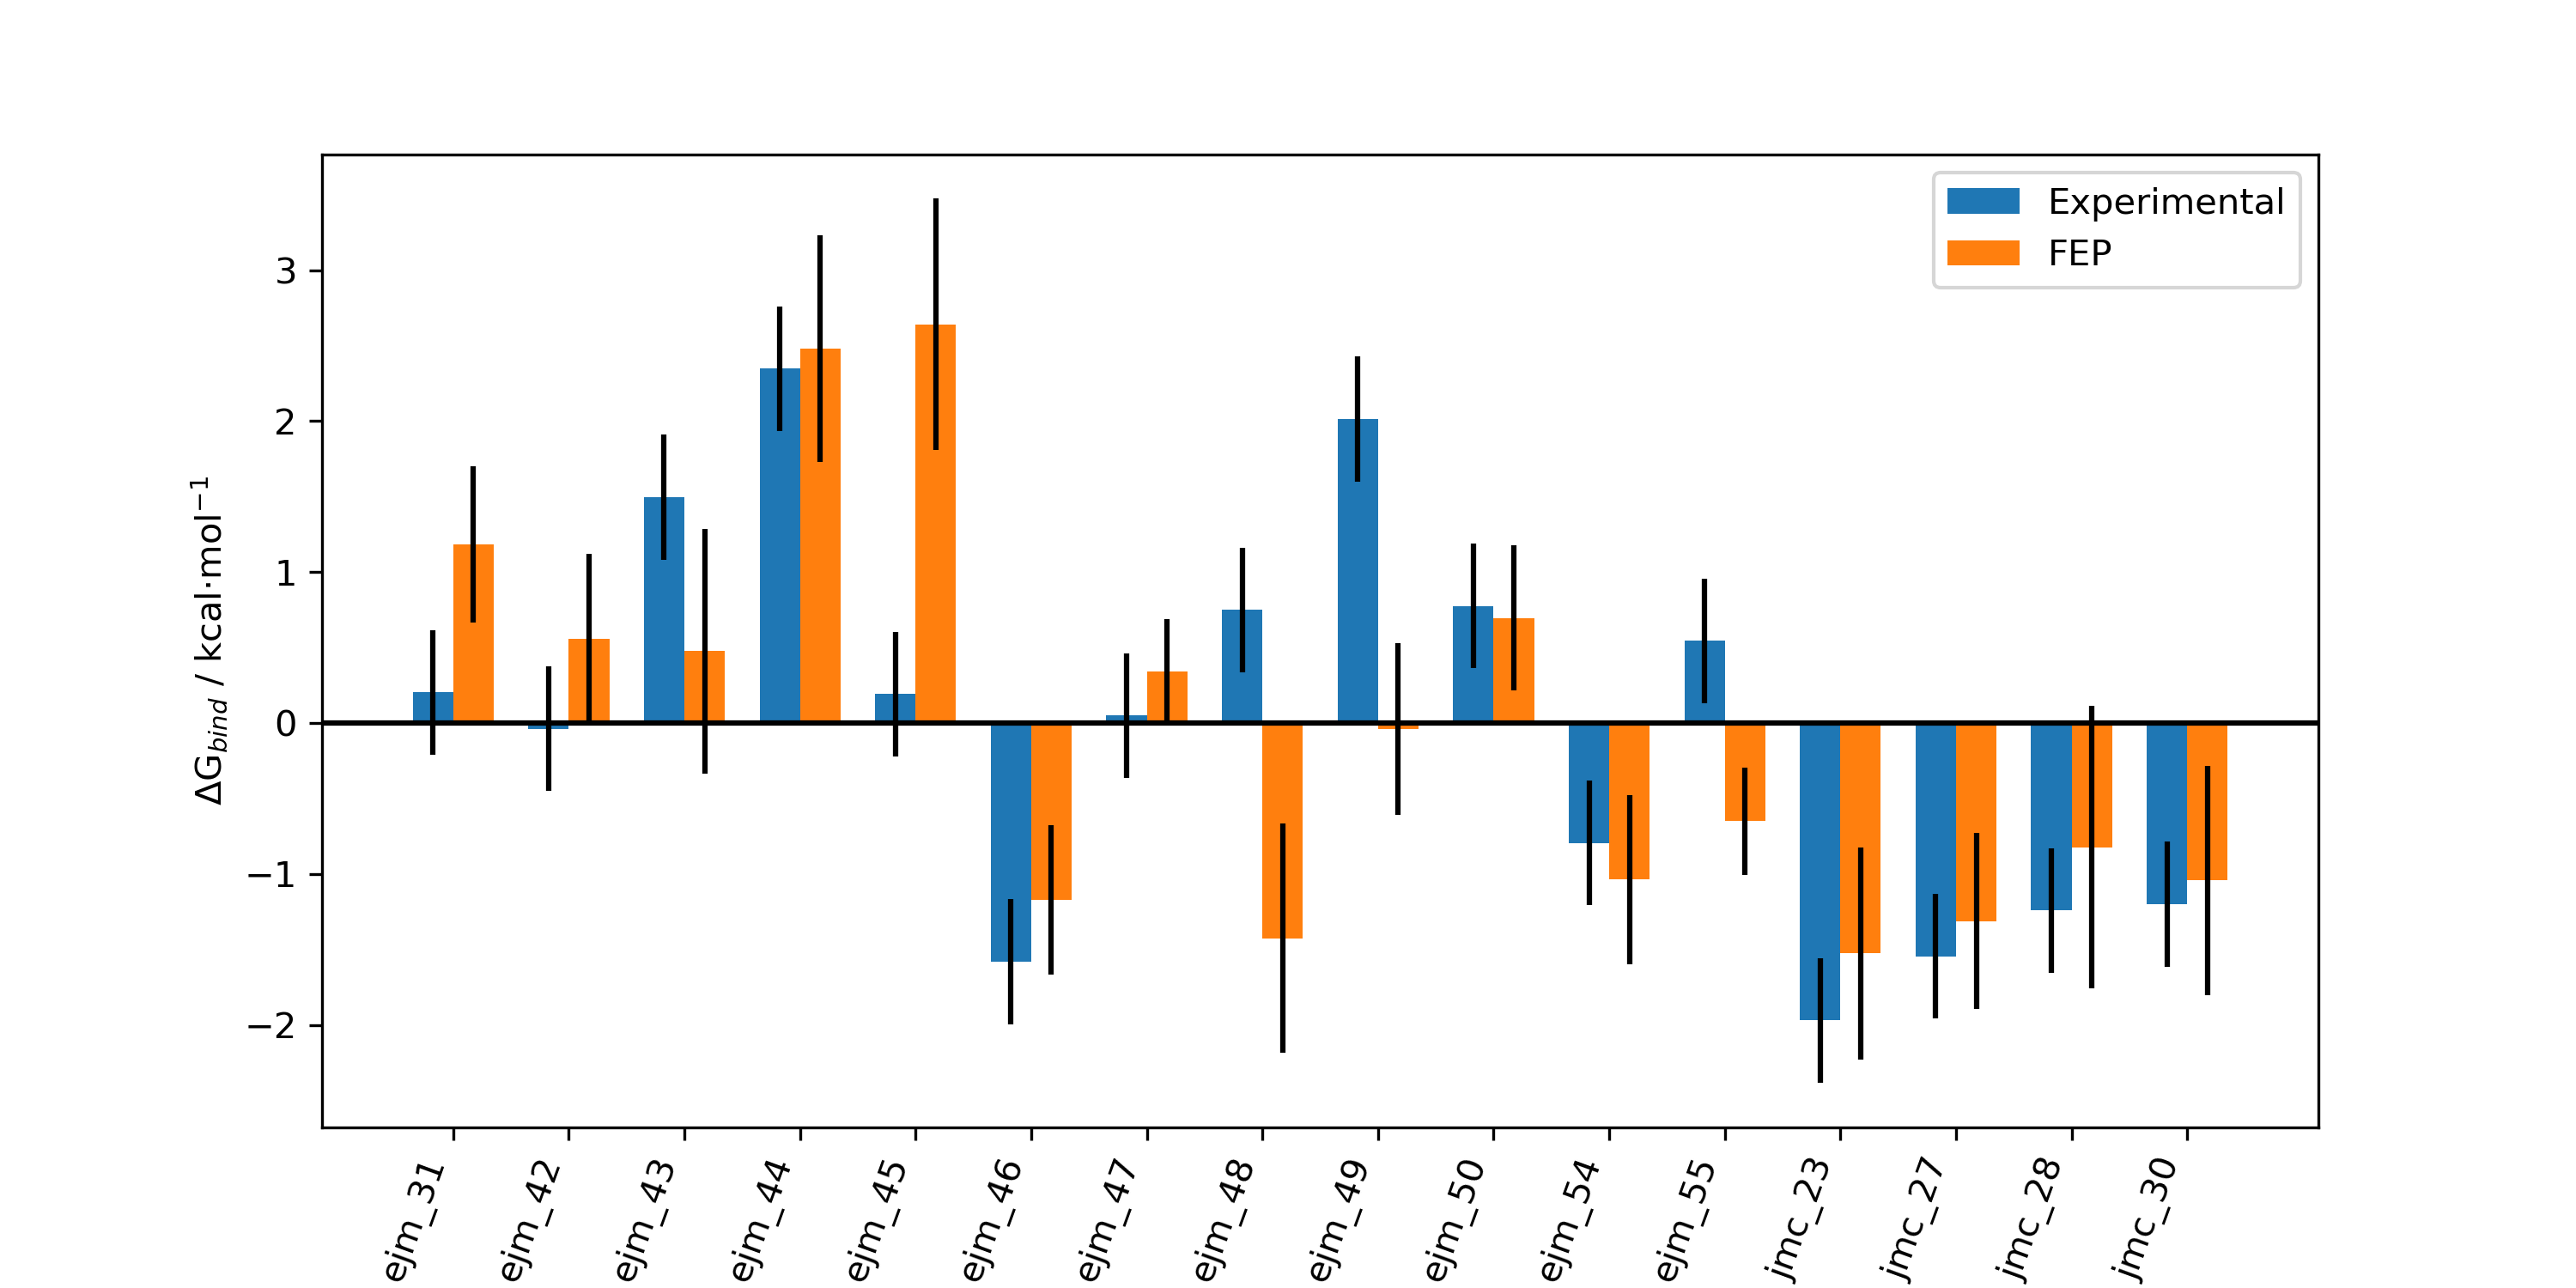
\includegraphics[width=\linewidth]{04_fep/inputs/tut_imgs/fep_barplot.png}
\caption{Example barplot depicting FEP results, generated with the analysis jupyter notebook included in this tutorial.}
\label{fep_barplot_fig}
\end{figure}



% %%%% YOU CAN USE THIS BLOCK FOR PYTHON:
% \begin{python}
% import numpy as np
    
% def incmatrix(genl1,genl2):
%     M = []
%     m = len(genl1)  # comment 
%     for i in m:
%         M.append(i)
    
%     return M
% \end{python}

% %%%% YOU CAN USE THIS BLOCK FOR BASH:
% \begin{lstlisting}
% $ command -arg1 -arg2 -arg3 -arg4 -arg5 -arg6 > output.file 2> err.file
% \end{lstlisting}

% %%%% YOU CAN USE THE SAME BLOCK FOR TEXT (e.g. STDOUT):
% \begin{lstlisting}[columns=flexible]
% this is an example of a message printed to StdOut!
% \end{lstlisting}

% %%%% FOR LARGE CHUNKS OF TEXTS, USE \scriptsize{} (OR EVEN \tiny{}) TO MAKE IT FIT THE COLUMNS
% {\scriptsize
% \begin{lstlisting}[columns=flexible]

% %VERSION  VERSION_STAMP = V0001.000  DATE = 06/30/15  11:44:23                  
% %FLAG TITLE                                                                     
% %FORMAT(20a4)                                                                   
% ACE                                                                             
% %FLAG POINTERS                                                                  
% %FORMAT(10I8)                                                                   
%     1912       9    1902       9      25      11      43      24       0       0
%     2619     633       9      11      24      13      21      20      10       1
%       0       0       0       0       0       0       0       1      10       0
%       0
% %FLAG ATOM_NAME                                                                 
% %FORMAT(20a4)                                                                   
% HH31CH3 HH32HH33C   O   N   H   CA  HA  CB  HB1 HB2 HB3 C   O   N   H   CH3 HH31
% HH32HH33O   H1  H2  O   H1  H2  O   H1  H2  O   H1  H2  O   H1  H2  O   H1  H2  
% O   H1  H2  O   H1  H2  O   H1  H2  O   H1  H2  O   H1  H2  O   H1  H2  O   H1  
% H2  O   H1  H2  O   H1  H2  O   H1  H2  O   H1  H2  O   H1  H2  O   H1  H2  O   
% H1  H2  O   H1  H2  O   H1  H2  O   H1  H2  O   H1  H2  O   H1  H2  O   H1  H2  
% O   H1  H2  O   H1  H2  O   H1  H2  O   H1  H2  O   H1  H2  O   H1  H2  O   H1  
% H2  O   H1  H2  O   H1  H2  O   H1  H2  O   H1  H2  O   H1  H2  O   H1  H2  O   
% H1  H2  O   H1  H2  O   H1  H2  O   H1  H2  O   H1  H2  O   H1  H2  O   H1  H2 
% \end{lstlisting}
% }


%\section{Checklists}
%Tutorials do not necessarily require the use of a checklist as in Best Practices documents; however, they can include these if desired.
%Several useful checklist formats are available, with examples presented in \texttt{sample-document.tex} in \url{github.com/livecomsjournal/article_templates/templates}.
%One example is shown here.
%
% Here is a single-column checklist that consists of multiple sub-checklists
%\begin{Checklists}
%
%\begin{checklist}{A list}
%\textbf{Single-column checklists are also straightforward by removing the asterisk}
%\begin{itemize}
%\item First thing let's do an item which breaks across lines to see how that looks
%\item Also remember
%\item And finally
%\end{itemize}
%\end{checklist}

%\begin{checklist}{Another list}
%\textbf{This is some further description.}
%\begin{itemize}
%\item First thing
%\item Also remember
%\item And finally
%\end{itemize}
%\end{checklist}
%
%\end{Checklists}








\section{Author Contributions}
%%%%%%%%%%%%%%%%
% This section mustt describe the actual contributions of
% author. Since this is an electronic-only journal, there is
% no length limit when you describe the authors' contributions,
% so we recommend describing what they actually did rather than
% simply categorizing them in a small number of
% predefined roles as might be done in other journals.
%
% See the policies ``Policies on Authorship'' section of https://livecoms.github.io
% for more information on deciding on authorship and author order.
%%%%%%%%%%%%%%%%
LH prepared Tutorial 1, DL and LH prepared Tutorial 2, AH and LH prepared Tutorial 3, JS, LH and JM prepared Tutorial 4. 
All authors contributed to manuscript writing. Authors are listed in alphabetical order, with the exception of the first co-author.
% We suggest you preserve this comment:
For a more detailed description of author contributions,
see the GitHub issue tracking and changelog at \githubrepository.

\section{Other Contributions}
%%%%%%%%%%%%%%%
% You should include all people who have filed issues that were
% accepted into the paper, or that upon discussion altered what was in the paper.
% Multiple significant contributions might mean that the contributor
% should be moved to authorship at the discretion of the a
%
% See the policies ``Policies on Authorship'' section of https://livecoms.github.io for
% more information on deciding on authorship and author order.
%%%%%%%%%%%%%%%
Gratitude is expressed to the users of BioSimSpace who have given important feedback over the past years that have influenced the production of our tutorials and documentation. 
% We suggest you preserve this comment:
For a more detailed description of contributions from the community and others, see the GitHub issue tracking and changelog at \githubrepository.

\section{Potentially Conflicting Interests}
%%%%%%%
%Declare any potentially competing interests, financial or otherwise
%%%%%%%
JM is a member of the Scientific Advisory Board of Cresset. 

\section{Funding Information}
%%%%%%%
% Authors should acknowledge funding sources here. Reference specific grants.
%%%%%%%
JM acknowledges support from an EPSRC standard grant (EP/P022138/1) and from the University of Edinburgh UCB via a an EPSRC-Impact Acceleration Account (IAA PIII074).

\section*{Author Information}
\makeorcid

\bibliography{references}

%%%%%%%%%%%%%%%%%%%%%%%%%%%%%%%%%%%%%%%%%%%%%%%%%%%%%%%%%%%%
%%% APPENDICES
%%%%%%%%%%%%%%%%%%%%%%%%%%%%%%%%%%%%%%%%%%%%%%%%%%%%%%%%%%%%

%\appendix


\end{document}